\icode[magenta]{N22E-ME-CA-L4-261019-001}
\nceeID[16]{2022湖北}{16}
打桩机是基建常用工具。某种简易打桩机模型如图所示，重物\(A\)、\(B\)和\(C\)通过不可伸长的轻质长绳跨过两个光滑的等高小定滑轮连接，\(C\)与滑轮等高(图中实线位置)时，\(C\)到两定滑轮的距离均为\(L\)。重物\(A\)和\(B\)的质量均为\(m\)，系统可以在如图虚线位置保持静止，此时连接\(C\)的绳与水平方向的夹角为\qty{60}{\degree}。某次打桩时，用外力将\(C\)拉到图中实线位置，然后由静止释放。设\(C\)的下落速度为\(\sqrt{\frac{3gL}{5}}\)时，与正下方质量为\(2m\)的静止桩\(D\)正碰，碰撞时间极短，碰撞后\(C\)的速度为零，\(D\)直向下运动\(\frac{L}{10}\)距离后静止(不考虑\(C\)、\(D\)再次相碰)。\(A\)、\(B\)、\(C\)、\(D\)均可视为质点。
\begin{enumerate}
	\item 求\(C\)的质量；
	\item 若\(D\)在运动过程中受到的阻力\(F\)可视为恒力，求F的大小；
	\item 撤掉桩\(D\)，将\(C\)再次拉到图中实线位置，然后由静止释放，求\(A\)、\(B\)、\(C\)的总动能最大时\(C\)的动能。
\end{enumerate}

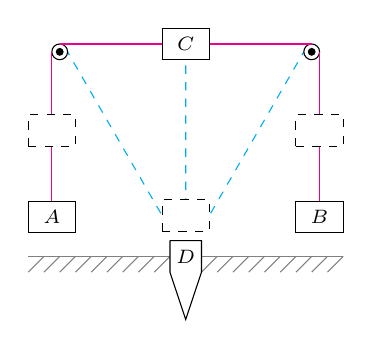
\begin{tikzpicture}[font=\scriptsize]
	\draw[dashed,cyan] (0,0)--(60:3) (0,0)--(120:3) (0,0)--(0,{3*sin(60)});
	\draw (1.6,{3*sin(60)}) circle(.1);
	\draw (-1.6,{3*sin(60)}) circle(.1);
	\fill (1.6,{3*sin(60)}) circle(.05) (-1.6,{3*sin(60)}) circle(.05);
	\draw[magenta] (1.6,{3*sin(60)+.1})--(-1.6,{3*sin(60)+.1}) (-1.7,{3*sin(60)})--(-1.7,.5) (1.7,{3*sin(60)})--(1.7,.5);
	\draw[draw=white,fill=white](-.3,0) rectangle(.3,.5);
	\draw[dashed,fill=white] (-.3,{0.3*sqrt(3)-.2}) rectangle(.3,{0.3*sqrt(3)+.2}) (-2,1.4) rectangle(-1.4,1.8) (1.4,1.4) rectangle(2,1.8);
	\draw[fill=white] (-.3,{3*sin(60)-.1}) rectangle(.3,{3*sin(60)+.3}) (-2,.3) rectangle(-1.4,.7) (1.4,.3) rectangle(2,.7);
	\draw[gray] (-2,0)--(2,0);
	\foreach \x in {-2,-1.8,...,1.8}
		\draw[gray] (\x,-.2)--++(.2,.2);
	\draw[fill=white] (-.2,.2)--(-.2,-.2)--(0,-.8)--(.2,-.2)--(.2,.2)--(-.2,.2);
	\node at(0,{3*sin(60)+.1}) {\(C\)};
	\node at(-1.7,.5) {\(A\)};
	\node at(1.7,.5) {\(B\)};
	\node at(0,0) {\(D\)};
\end{tikzpicture}
\begin{answer}
    
\end{answer}